
\section{Introduction}


\begin{figure}[ht!]
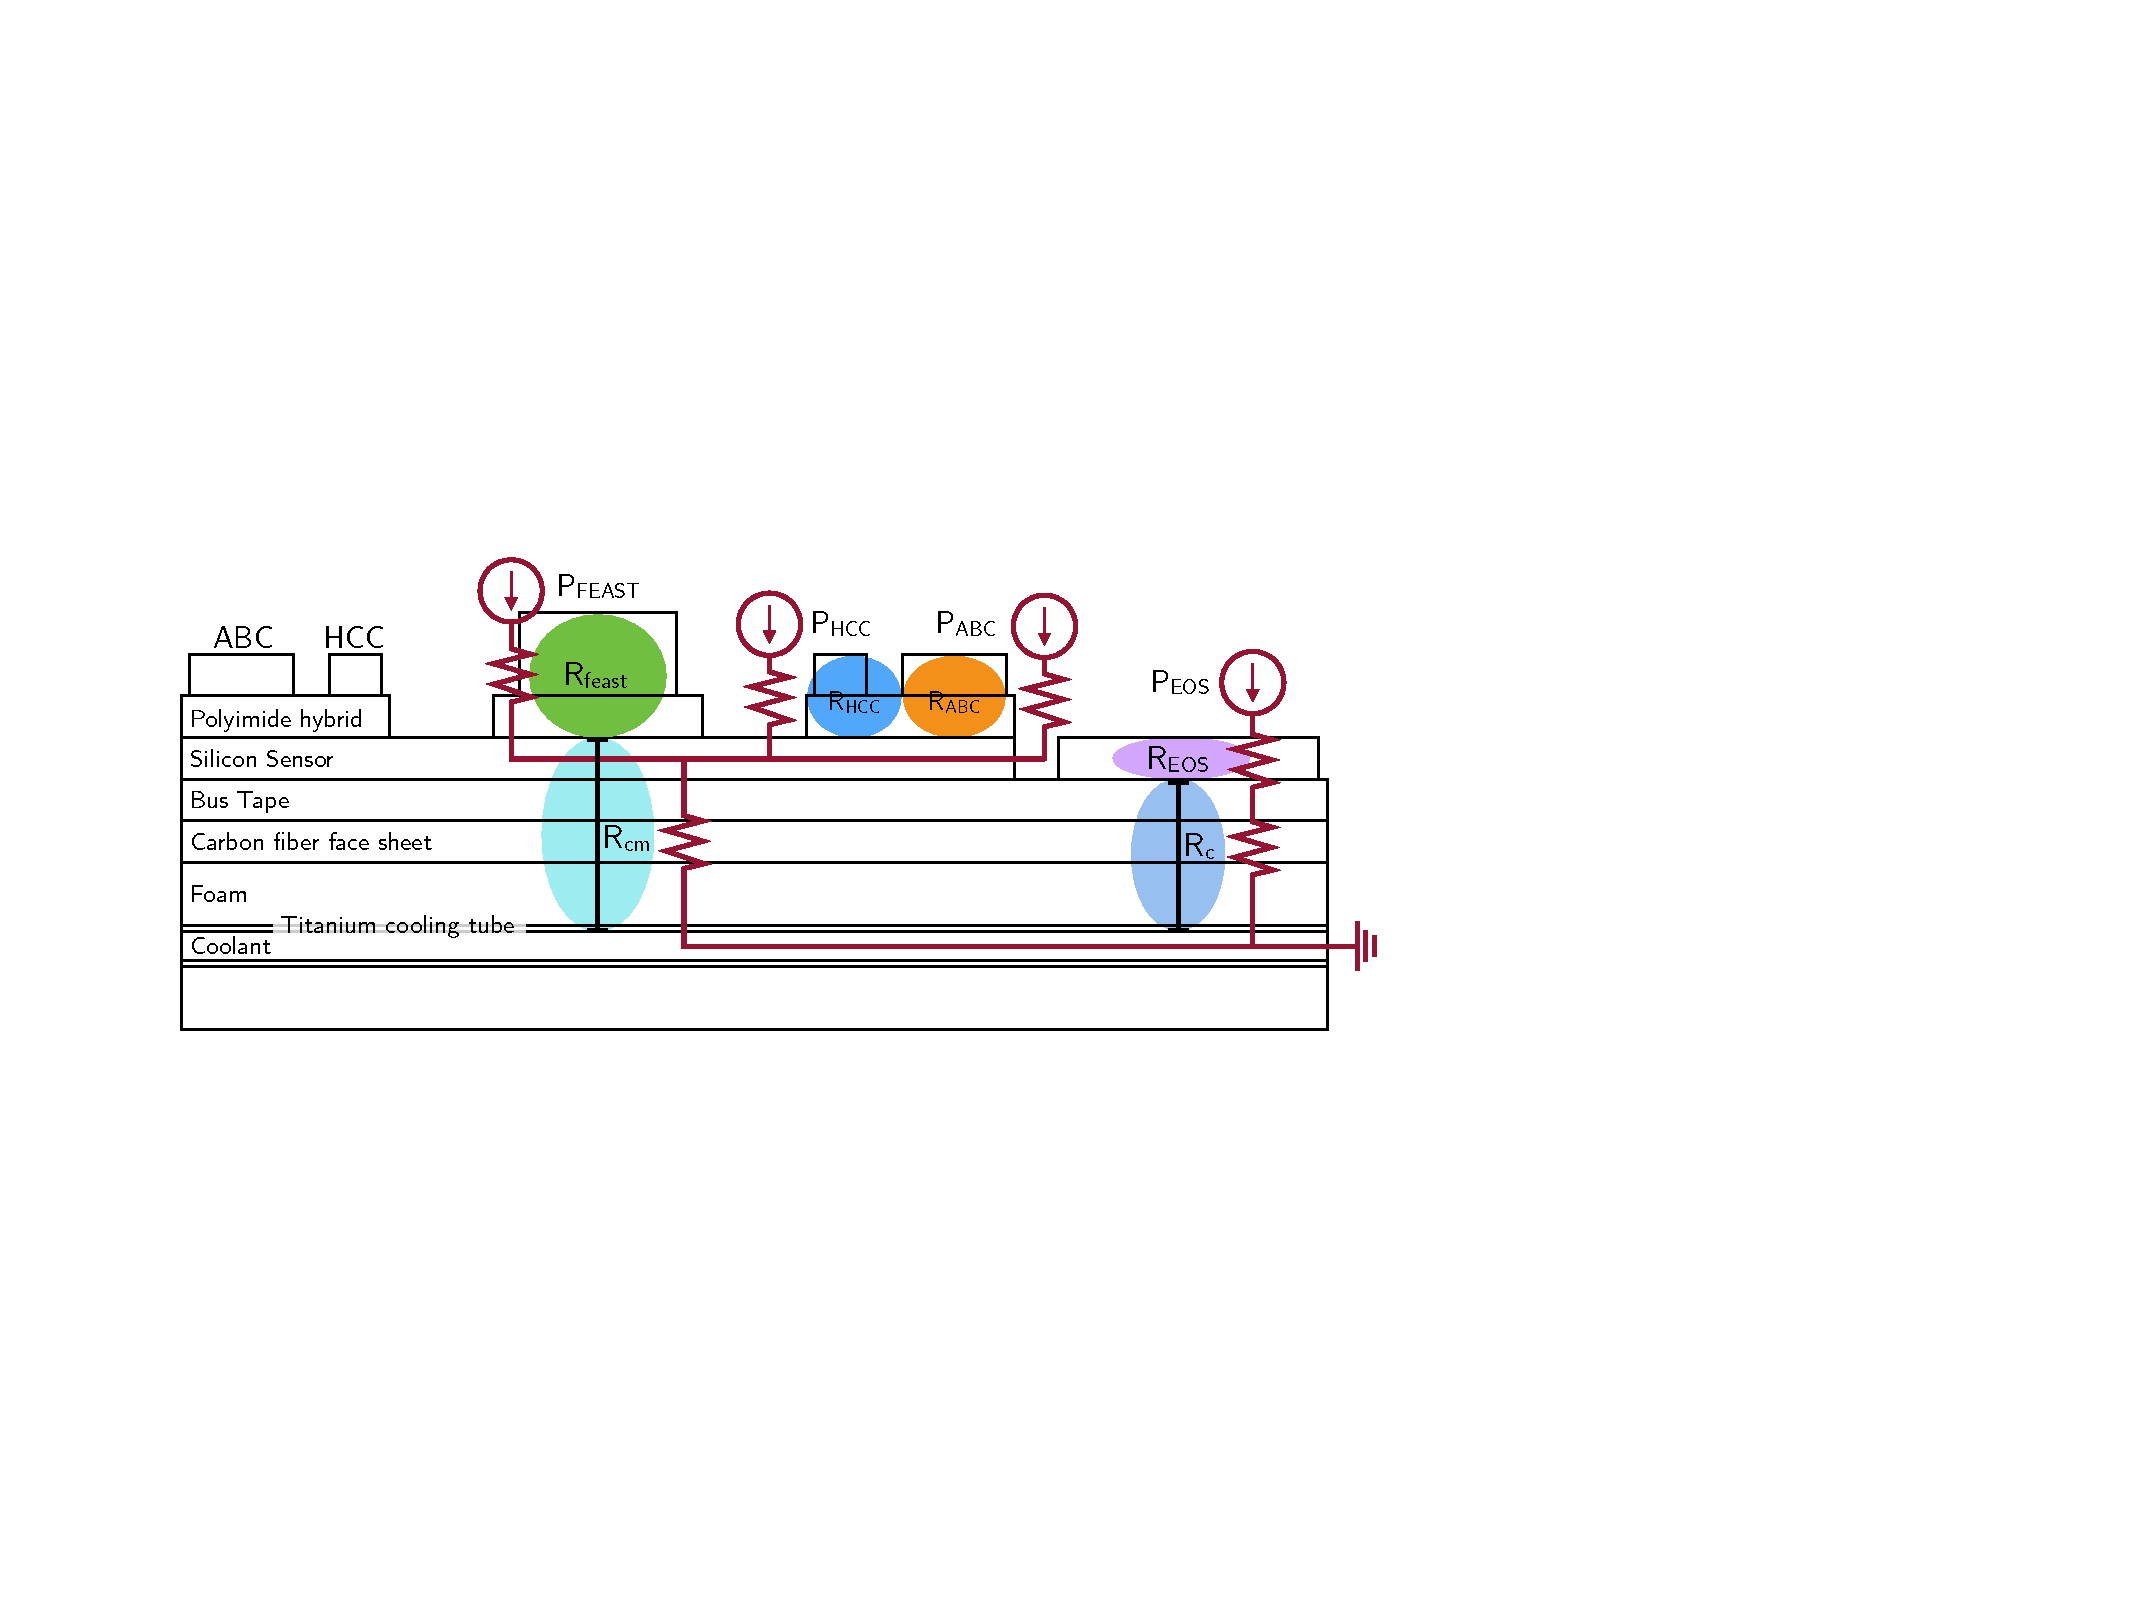
\includegraphics[width=.99\textwidth]{figures/thermoelectric_model.pdf}
\caption{
The thermo-electric model, its analogy with electrical circuits, and definitions of terms.
}
\label{thermoelectric_model}
\end{figure}

Note that e.g. all ABCs are treated as a single node in this description, meaning the ABC power refers
to the total power in all ABCs, and the thermal resistance is an effective thermal resistance for all
ABCs (the same applies to the FEAST and HCC).

Note that the effect of the AMAC as a power source affecting the module temperature is neglected in
the following; however, the AMAC represents roughly 1\% of the total module power, so the impact on
the temperatures of the module is negligible. (The AMAC power itself is counted as part of the total
module power.)

The pathway shared by the EOS and the other components is called $R_{C}$, and is also fit using the
data by measuring the temperature. The two are related according to $R_{CM} = R_C + R_M$.
